\documentclass{llncs}

\usepackage[unicode=true,hidelinks]{hyperref}
\usepackage{graphicx}

\begin{document}

\title{An Architecture Pattern for Network Resilient Web Applications}

\author{Julien Richard-Foy\and Olivier Barais \and Jean-Marc J\'ez\'equel\\{\tt \{first\}.\{last\}@irisa.fr}}

\institute{IRISA, Universit\'e de Rennes, France}

\maketitle

\begin{abstract}
With the advent of Internet connected mobile devices having a an intermittent network connection rises the need for a good support of network resilience for Web applications. Achieving resilience requires to resite the application logic execution on client-side when network failures are detected and then to synchronize changes to the server when the connection is back. These failures can happen on each possible user action, making resilience a cross-cutting concern, and therefore making it hard to isolate in the application's code. This paper presents an architecture pattern based on event sourcing isolating the network resilience concern. Applications built on top of this architecture pattern keep delivering a good quality of experience under bad network conditions. We implemented two example applications and captured the client-server synchronization logic as a reusable library.
\end{abstract}

\section{Introduction}

Web applications work only as long as the network connection and the server are up. If the network connection or the server is down, applications may suffer from inconsistency, freeze or latency, resulting in a bad user experience. With the advent of Internet connected mobile devices (smartphones and tablets) rises the need for a good support of an off-line mode for Web applications.

In this paper, we use the term \textit{resilience} to refer to the ability of a Web application to deliver a good Quality of Experience (QoE) under bad network conditions. The resilience level can vary. For instance, when an application detects a network failure, it can either:

\begin{itemize}
 \item Display an error message informing the user that its last action failed (\textit{e.g.} Trello\footnote{\href{http://www.trello.com}{http://www.trello.com}});
 \item Fallback to a read-only mode (\textit{e.g.} Google Drive\footnote{\href{http://drive.google.com}{http://drive.google.com}});
 \item Let the user work and try to synchronize the changes when the connection is back (\textit{e.g.} Workflowy\footnote{\href{http://www.workflowy.com}{http://www.workflowy.com}}).
\end{itemize}

To keep delivering a good QoE when the server is unreachable, the application must resite the business logic on the client-side and then synchronize the changes to the server when the connection comes back. According to the application's domain this task can be more or less hard to achieve. Typically, if the logic needs to access to a large amount of data (\emph{e.g.} a search engine) or to perform a heavy computation, the price to pay may be too high for the client. However, in all other cases (examples???) the client could take on the business logic execution. Nevertheless, the need for detecting and handling network failures on all user actions makes resilience a cross-cutting concern~\cite{Kiczales97_AOP}, and makes it hard to isolate in the application's code.

This article presents an architecture pattern based on event sourcing to isolate the resilience concern in Web applications. Our pattern is agnostic to the whole application architecture, it requires little adaptation for existing applications to use it, it only isolates the client-server execution distribution policy and allows applications to deliver a good QoE when the network is down.

Based on this architecture pattern we captured the client-server synchronization logic as libraries for both the server and client sides, and used it to develop two use case applications.

\section{Related Work}

\paragraph{Cloud Elasticity} Zhang \emph{et. al.} presented an application model augmenting the computing power of resource-constrained mobile devices~\cite{Zhang10_ElasticMobile}.

\paragraph{Offline Support}

Requirements and mechanisms for supporting offline mode in client-server applications have been addressed in 2000 by Yang \emph{et. al.}~\cite{Yang2000_OfflineMode}.

More recently, Marco \emph{et. al.}~\cite{Marco11_InterruptionResilience} and Kao \emph{et. al.}~\cite{Kao12_WOPRE} presented runtime environments making Web applications available even when offline. Their runtime environment also features content adaptation, according to the device bandwidth or computing capabilities.

\paragraph{Persistent Resources}

Cannon \emph{et. al.} showed how to get Web application working offline using persistent resources~\cite{Cannon10_Persistence}. This approach is \emph{data centric}: data objects are enhanced with a persistence and synchronization mechanism so that they automatically keep track of their changes and synchronize themselves to a server.

\cite{Benson10_SyncKit}

\paragraph{Event sourcing}

Event sourcing ``captures all changes to an application state as a sequence of events''~\cite{Fowler05_ES}. Event sourcing is mostly used in conjunction with command and query segregation in order to solve scalability problems~\cite{Betts13_CQRS}.

\section{Contribution}

Our architecture relies on the idea of event sourcing: the state of the application is determined by the application of a succession of events. For instance, in the case of a text editor, such events could be text insertion and text deletion. Events are just described by data: \emph{e.g.} the position and the inserted character.

Essentially, the idea of our architecture is to store the events corresponding to each performed action in a queue on client-side, and to synchronize the queue content when the network connection is up. The business logic corresponding to each event is always executed on client-side so users do not suffer from latency when they interact with the application. Finally, on server-side, the events are stored in a log.

\begin{figure}
\centering
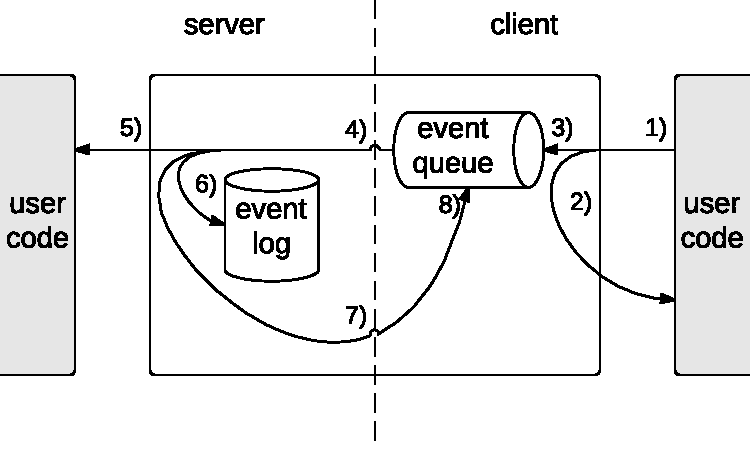
\includegraphics[width=8cm]{arch.pdf}
\caption{Architecture}
\label{fig-arch}
\end{figure}

Figure \ref{fig-arch} depicts the process involved when an user performs an action in the application. The application code is partitioned between the client and server sides, with a synchronization module in between. The left and right parts, in gray, represent the application code, and the central part represents the synchronization module. The process involved when a user performs an action is the following:

\begin{enumerate}
 \item A domain event corresponding to the user action is created on the client and sent to the synchronization module~;
 \item The synchronization module on client-side calls back the logic defined by the application for this event~;
 \item The event is put into an event queue~;
 \item If the network connection is up, the queue content is sent to the server side part of the synchronization process~;
 \item On server-side, the synchronization module invokes the business logic defined by the application for this event~;
 \item The event is stored in an event log on the server side~;
 \item The application of the event is acknowledged to the client~;
 \item The client removes the acknowledged event from its queue.
\end{enumerate}

With this design, users have an instant feedback for their actions because their logic is executed on client-side.

% \begin{figure}
% \centering
% 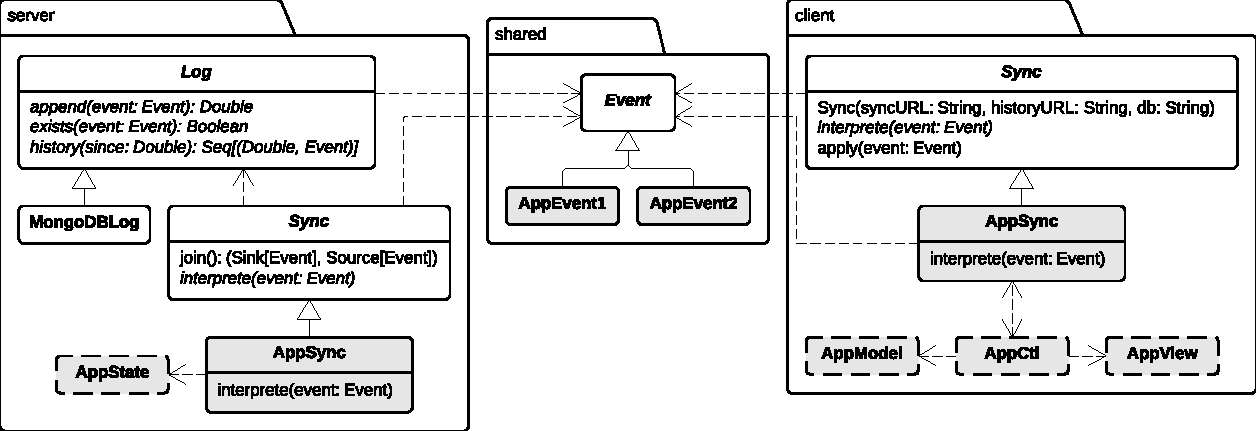
\includegraphics[width=18cm,angle=90]{classes.pdf}
% \caption{Architecture}
% \label{fig-classes}
% \end{figure}

\begin{figure}
\centering
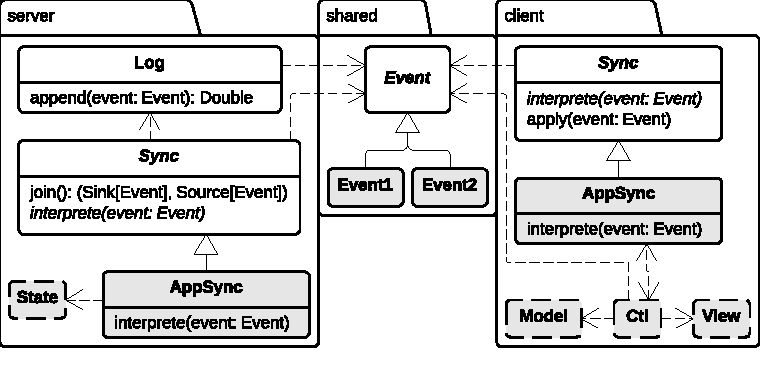
\includegraphics[width=12cm]{classes2.pdf}
\caption{Architecture}
\label{fig-classes-2}
\end{figure}

Figure \ref{fig-classes-2} shows a class diagram of our architecture pattern. Classes in gray are those written by users, classes in white are provided by our library. The application defines the {\tt Event1} and {\tt Event2} domain events and implements the business logic corresponding to their interpretation on client-side and server-side (methods {\tt interprete} of classes {\tt server.AppSync} and {\tt client.AppSync}, respectively). When an user performs an action the {\tt client.Sync\#apply} method is called, which calls back the logic implemented in {\tt client.AppSync.interprete}, put the event in its queue and tries to synchronize the queue to the server. On server-side, the {\tt server.Sync.join()} method is called when a client joins the application, it returns both a sink and a source of events. The sink is used when events are received from a client and the source is used to notify a client that an event has been logged. When an event is pushed to the sink, the {\tt 
interprete} method is called, applying the business logic corresponding to the event, the event is appended to a log (class {\tt Log}), and pushed back to the client \emph{via} the source. The classes drawn with dotted lines are not part of the architecture pattern, they are given here as an illustration of a possible integration with the whole application. Here, we have a class {\tt State} on server-side, keeping an in-memory state of the system, and classes {\tt Model}, {\tt Ctl} and {\tt View} on client-side, following a kind of model-view-controller pattern.

\paragraph{Communication between roles}

\begin{figure}
\centering
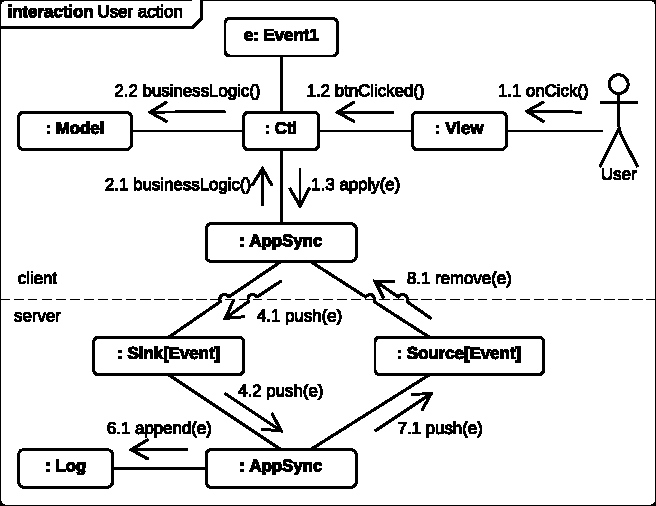
\includegraphics[width=10cm]{communication.pdf}
\caption{Architecture}
\label{fig-communication}
\end{figure}

Figure \ref{fig-communication} depicts the interactions between the different components of the architecture when a user performs an action.

\section{Validation}

\subsection{Samples implementation}

We implemented the following sample applications:

\paragraph{TodoMVC} The famous TodoMVC~\footnote{\href{http://todomvc.com/}{http://todomvc.com/}} application compares frameworks for interactive Web applications development. Our implementation works both online and offline and automatically synchronizes its state when the network connection is up.

\paragraph{Notes} We also implemented a simple text editor that works online and offline and synchronizes its state when the network connection is up.

\paragraph{}The synchronization logic is completely captured and reused by each sample.

\subsection{Extensibility}

\subsection{Integration in existing applications}

\subsection{Limitations}

\paragraph{Snapshots}

\paragraph{Collaboration}

\section{Discussion}

Network resilience is a valuable property in a world of intermittently connected mobile devices. However, engineering network resilient software is challenging because resilience is a cross-cutting concern. In this paper we presented an architecture pattern isolating this concern. We implemented a library, based on this architecture pattern, capturing the client-server synchronization logic. Future work will handle concurrent users.

\bibliographystyle{plain}
\bibliography{references}

\end{document}
